\chapter{Risultati e Conclusioni}
L'obbiettivo della valutazione del sistema in situazioni realistiche, quello di dare una prova anche se vaga di funzionamento. 
I risultati della valutazione sono stati confrontati.
\begin{figure}[h]
	\centering
		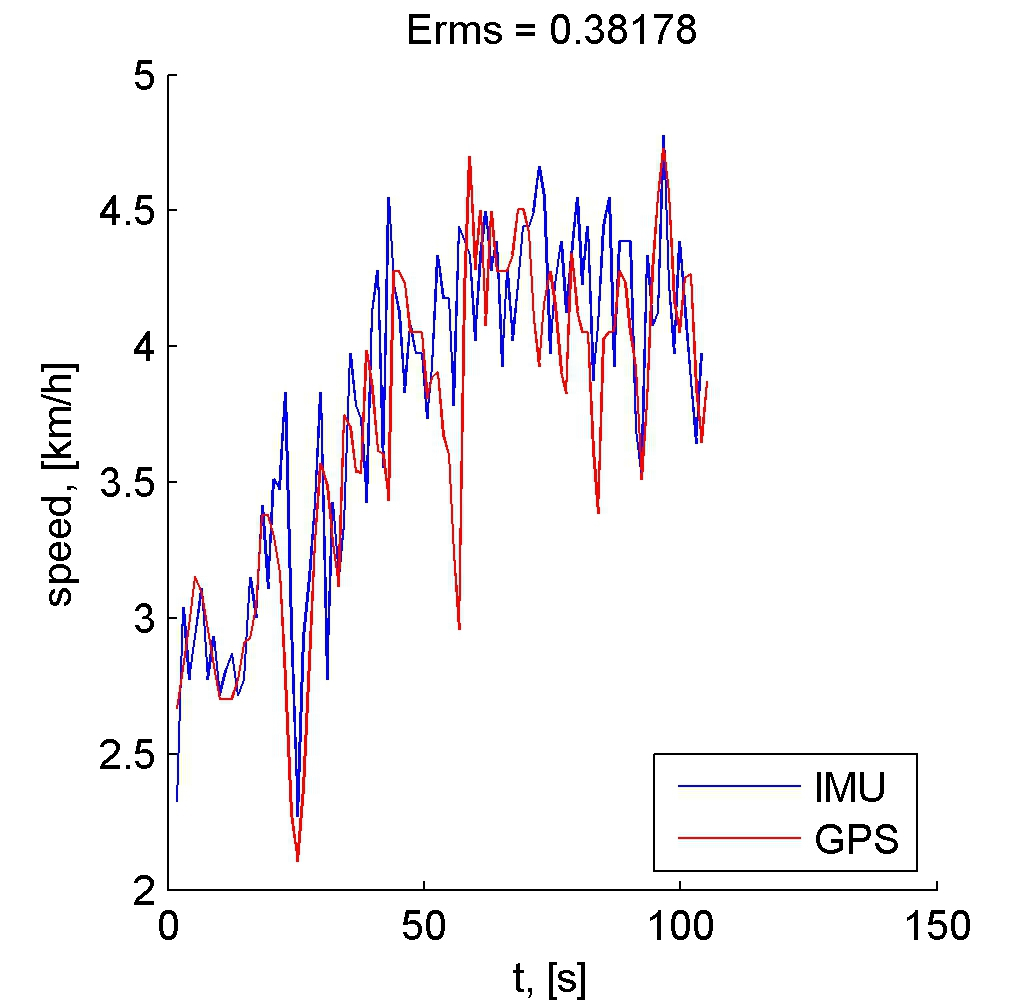
\includegraphics[width=.8\textwidth]{imgs/speedSVR4.jpg}
	\caption{Confronto fra le due velocit� $IMUspeed$ (traccia rossa) e $GPSspeed$ (traccia blu) rispetto al tempo in $Km/h$ in funzione del tempo in secondi. Mostra una forte somiglianza tra tra le due velocit�.}
	\label{fig:IMUspeedGPSspeedVStime}
\end{figure}
\begin{figure}
	\centering
		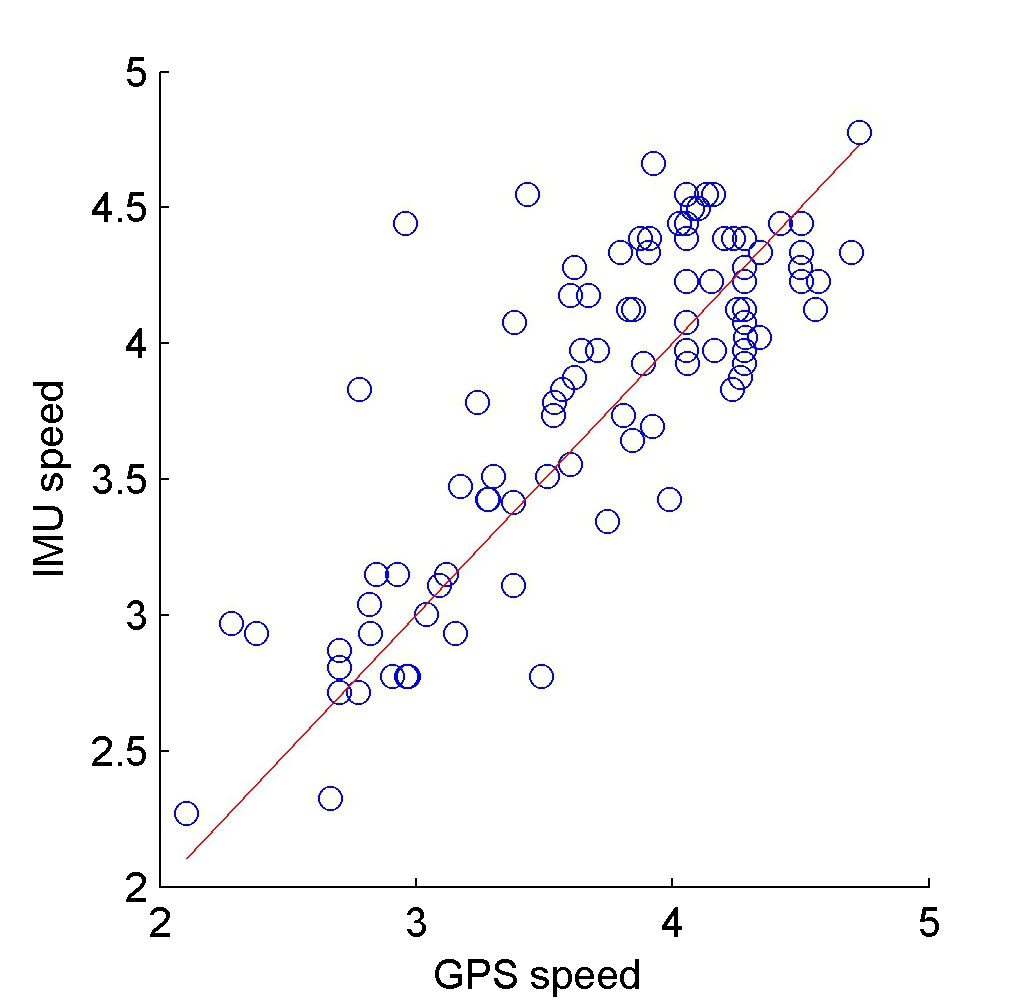
\includegraphics[width=.8\textwidth]{imgs/speedSVR5.jpg}
	\caption{Grafico a dispersione (\textit{scatter plot}) delle due velocit� $IMUspeed$ e $GPSspeed$. Mostra come ci sia una buona corrispondenza fra i due gruppi di valori.}
	\label{fig:IMUspeedVSGPSspeed}
\end{figure}

\begin{figure}
	\centering
		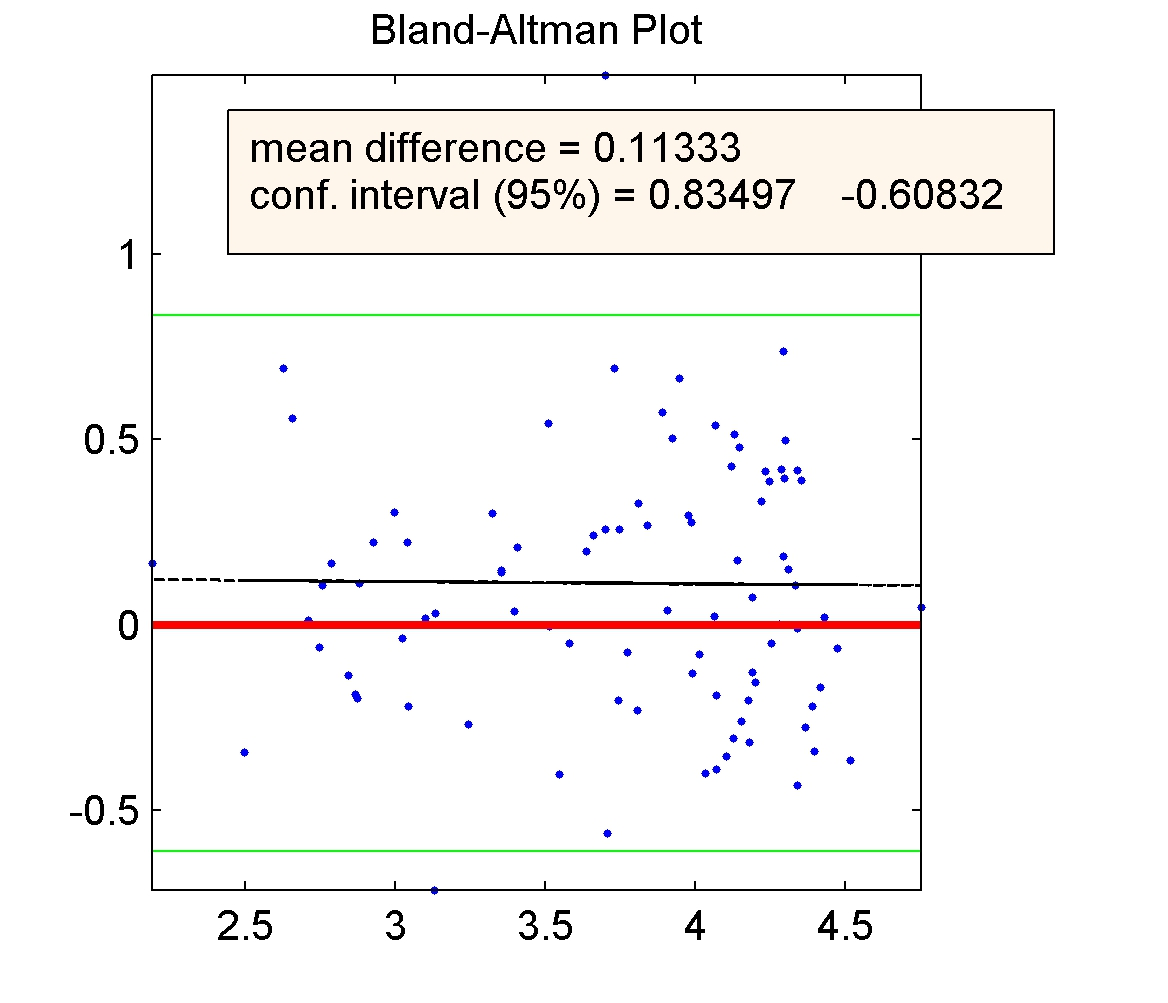
\includegraphics[width=.8\textwidth]{imgs/speedSVRBlandAltmann.jpg}
	\caption{Confronto fra le due velocit� $IMUspeed$ e $GPSspeed$ mediante un Bland Altman \textit{plot} o grafico a differenza o grafico delle differenze medie. La linea rossa rappresenta la linea a differenza nulla, la linea nera la differenza media, mentre le linee verdi la deviazione standard (o intervallo di confidenza). Il 95\% dei valori sta all'interno dell'intervallo di confidenza. }
	\label{fig:IMUspeedVSGPSspeedBA}
\end{figure}

\begin{figure}
	\centering
		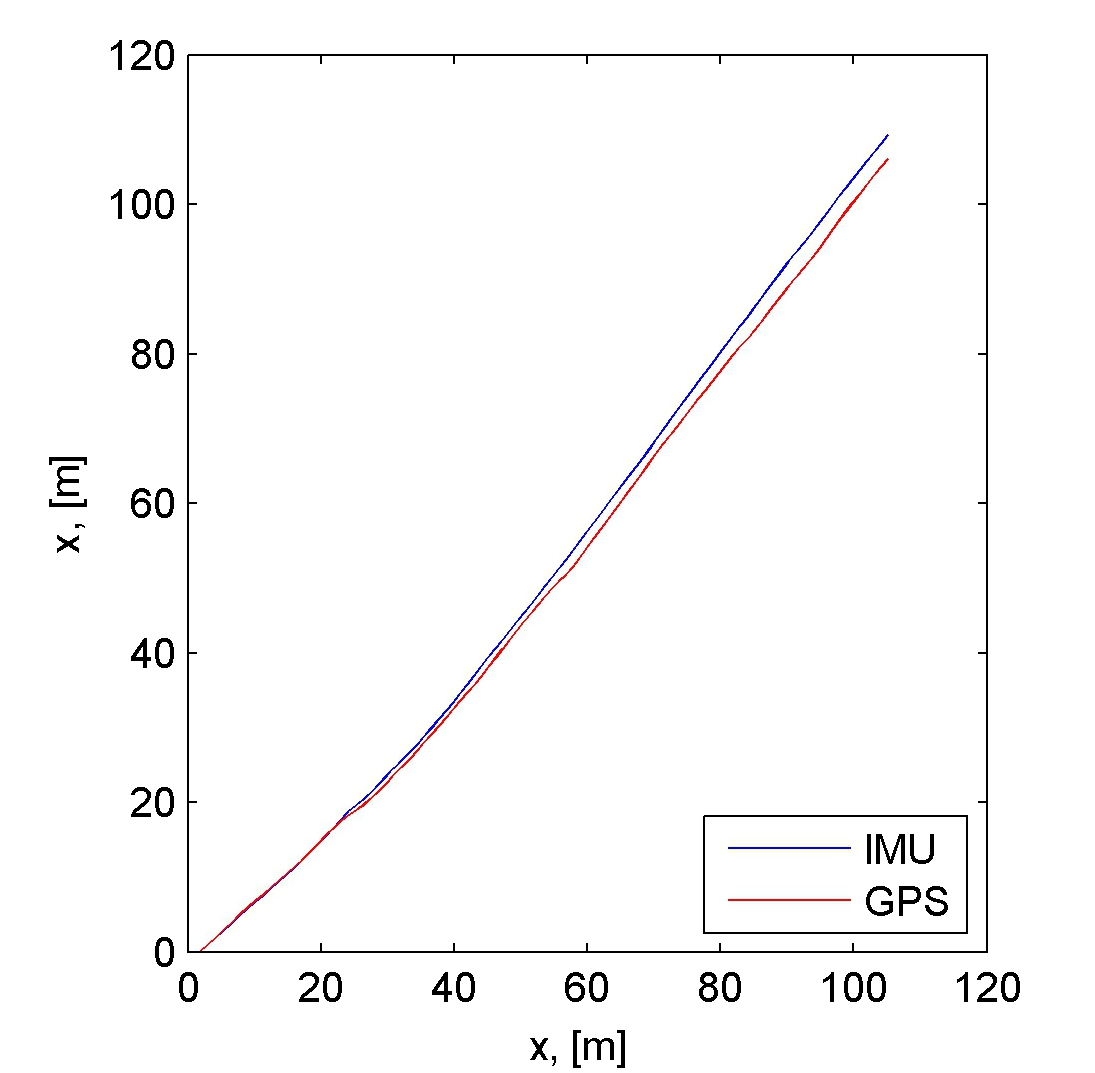
\includegraphics[width=.8\textwidth]{imgs/displSVR1.jpg}
	\caption{Confronto fra le due distanze $IMUdistance$ (traccia blu) e $GPSdistance$ (traccia rossa) rispetto al tempo. Mostra che la IMU sovrastima la distanza. Al termine dell'esperimento (a circa $110m$ di distanza percorsa) l'errore � commesso � di circa $5m$.}
	\label{fig:IMUdistanceGPSdistanceVStime}
\end{figure}

\begin{figure}
	\centering
		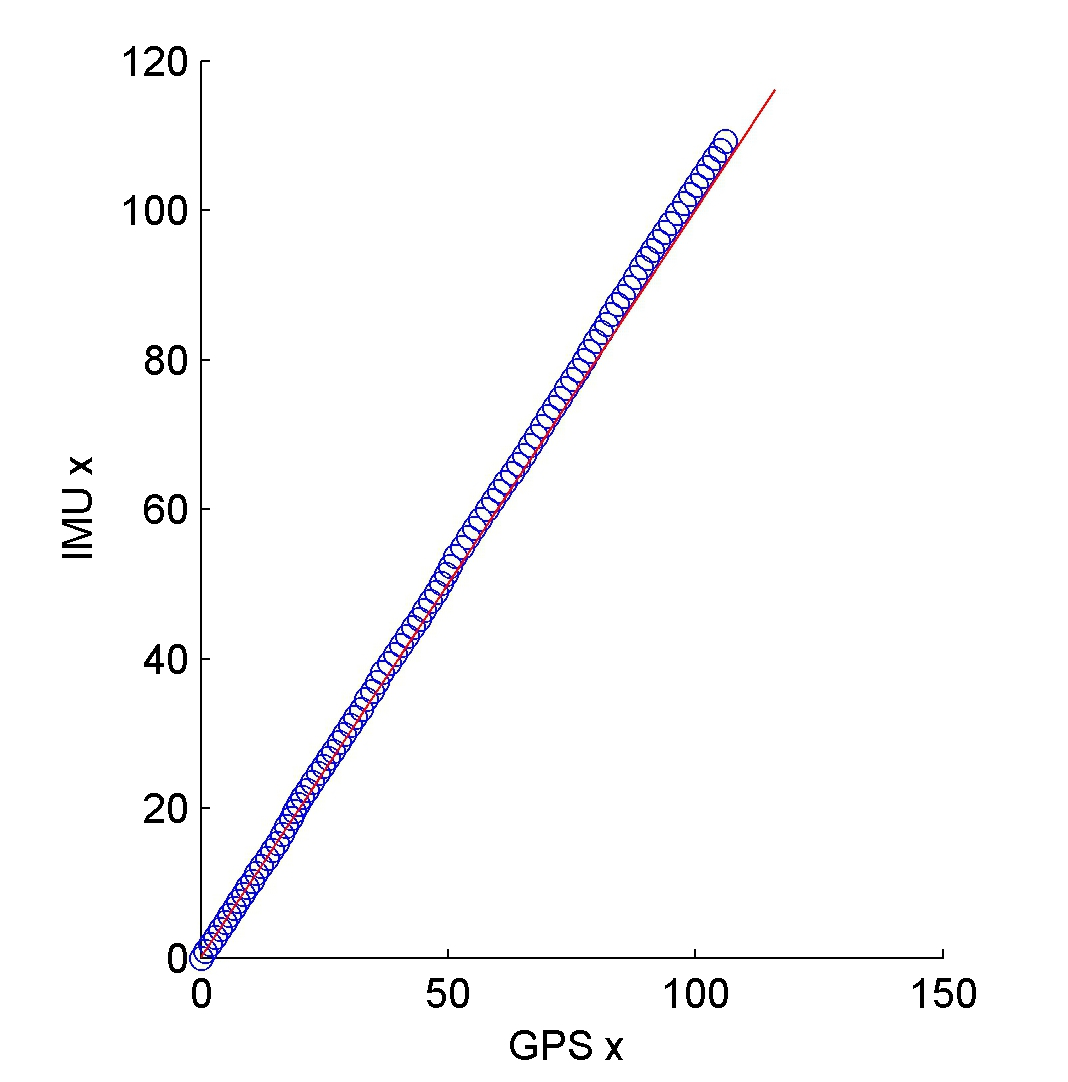
\includegraphics[width=.8\textwidth]{imgs/displSVR2.jpg}
	\caption{Grafico a dispersione delle due distanze $IMUdistance$ e $GPSdistance$ mostra una elevato grado di allineamento fra le distanze misurate con i due strumenti.}
	\label{fig:IMUdistanceVSGPSdistance}
\end{figure}

Per concludere, in questo lavoro � stato affrontato il problema della segmentazione del segnale giroscopico (con un giroscopio posizionato sul collo del piede) prodotto della deambulazione umana, mediante l'algoritmo di Viterbi, su un'HMM minimale a 4 stati, addestrato con Apprendimento Supervisionato su un \textit{training set} etichettato mediante stereofotogrammetria Vicon\tm. Il sistema di segmentazione � stato quindi implementato con una versione in linea dell'algoritmo di Viterbi su uno \textit{Smartphone} Android. Infine � stato ideato un meccanismo di verifica del funzionamento del sistema, basato sul confronto della velocit� calcolata mediante il sistema e quella calcolata da un dispositivo GPS.\\
Il sistema fornisce un surrogato inerziale temporaneo al sistema GPS per quanto riguarda il calcolo della distanza. Vale a dire, che dato che il sistema GPS pu� incappare in problemi di assenza di segnale, il sistema pu� subentrare nella misurazione della distanza per brevi periodi di tempo (per adesso un paio di minuti) ed essere sostituito dal GPS, quando il segnale � nuovamente disponibile. Il vantaggio della misurazione inerziale della distanza sul modello di misurazione mediante GPS � la sua autonomia, infatti funziona anche al chiuso. Il suo svantaggio � invece il fatto che sia inaccurata. Sviluppi futuri del lavoro dovranno pensare al miglioramento del modello con HMM ad emissioni a misture di densit� gaussiane multivariate. Ci� migliorerebbe sicuramente le prestazioni del sistema sulla capacit� di segmentazione del sistema.\\
Un secondo sviluppo futuro del lavoro � quello di progettare con lo stesso meccanismo modelli di semplici attivit� quotidiane, come la corsa, salire dei gradini, sedersi, alzarsi e cos� via, ed 

 